\chapter{Overfitting}\label{chap:overfitting}

\section{Begriffserklärung}\label{sec:what-is-overfitting}

Genaue Daten über Krankheitsbefälle im Agrarsektor sind rar, da diese in der Regel nicht öffentlich zugänglich sind.\footnote{Datenschutz kann ein Grund dafür sein.}  Daher musste mit \textit{Overfitting} gerechnet werden. Das künstliche neurale Netzwerk soll daraufhin trainiert werden, dass es möglichst alle Befälle, die untersucht werden, erkennt. Dafür wird es im ersten Schritt mit einem Trainingsdatensatz trainiert. Im folgenden Schritt mit einem kleineren Validierungsdatensatz überprüft, wie gut das Netz trainiert wird. Overfitting tritt auf, wenn das Netz auf die Daten aus dem Trainingsdatensatz mit sehr hoher Erfolgsquote erkennt, jedoch vergleichsweise schlechte Ergebnisse bei der Validierung bzw. bei unbekannten Daten erzielt. Das geschieht, weil sich das Netz auf nicht relevante Datenpunkte konzentriert, die im nur Trainingsdatensatz auftreten, aber nicht die allgemeine Charakteristika der Objekte widerspiegeln. 
\\\\
\begin{figure}[ht]
  \centering
  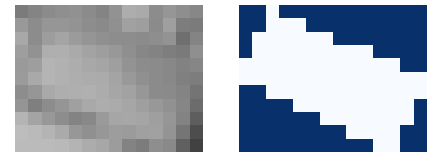
\includegraphics[height=2.5cm]{pics/mask.png}
  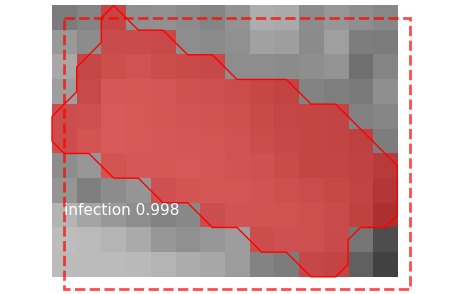
\includegraphics[height=2.5cm]{pics/pred.png}
  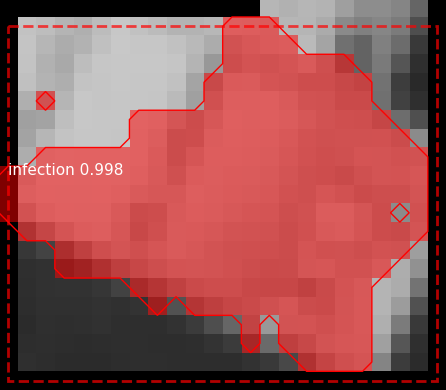
\includegraphics[height=2.5cm]{pics/bad-pred.png}
  \caption[Beispiel Overfitting]{V.l.n.r. Bild von infizierter Agrarfläche aus Trainingsdatensatz / Binärmaske der infizierten Region, wird gemeinsam mit dem linken Bild zum Training in das KNN gespeist / Selbiges Bild, Ergebnis nach Trainingsdurchlauf, prognostizierte Ergebnisfläche in rot / Bild der selben Fläche, was nicht aus dem Trainingsdatensatz stammt, prognostizierte Ergebnisfläche in rot}
  \label{fig:example-overfitting}
\end{figure}
\noindent
In Abb. \ref{fig:example-overfitting} ist ein Beispiel wie Overfitting sich auswirken kann. Die linken zwei Bilder sind ein exemplarischer Auszug aus dem Trainingsdatensatz. Einmal eine visuelle Repräsentation der NDVI-Werte der infizierten Agrarfläche und die Binärmaske, welche die infizierte Fläche markiert. Das selbe Bild wurde nach einem erfolgreichen Trainingsdurchlauf der Mask R-CNN-Implementierung übergeben und es hat den erkrankten Bereich nahezu perfekt erkannt. Das vierte Bild zeigt zentriert das selbe Feld. Jedoch ist der Ausschnitt größer, rotiert und die Aufnahme stammt von einem anderen Datum.\todo{Genaues Datum nötig?} Der Prognose zur Folge ist die Infizierung auf die benachbarten Felder übergesprungen, was nicht der Realität entspricht. Overfitting ist ein bekanntes Problem im Bereich des maschinellen Lernens und es existieren multiple Methoden, um dem entgegenzuwirken.

\section{Data Augmentation}\label{sec:augmentation}

Generell ist ein sehr großer Datensatz ($\ge10000$ Elemente) für das Training förderlich. Jedoch ist das nicht immer möglich. In diesem Fall kann der Datensatz künstlich durch \textit{Data Augmentation} vergrößert werden. Zu Data Augmentation zählen geringe Veränderungen der Daten - hier Bildmanipulationen. Solche Operationen können unter anderem
\begin{itemize}
	\item Rotationen,
	\item Spieglungen,
	\item Translationen,
	\item zufällige Ausschnitte,
	\item Gauß'sches Rauschen,
	\item Helligkeitsveränderungen,
	\item oder Kombinationen davon
\end{itemize}
beinhalten. Wobei nicht jede Augmentation-Technik für jeden Anwendungsfall sinnvoll ist. Wenn zum Beispiel ein KNN auf Autoerkennung trainiert werden soll, ist es nicht nützlich oder sogar hinderlich die Bilddaten so zu rotieren, dass es von oben nach unten oder umgekehrt zeigt. Des weiteren ist sinnvoll Data Augmentation einzusetzen, obwohl genügend Daten vorhanden sind. So besteht der Datensatz aus zwei Klassen von Autos, Marke A und Marke B. Die Front der Fahrzeuge der Marke A sind nach rechts ausgerichtet, während die Autos der Marke B nach links ausgerichtet sind. Das neuronale Netz wird diesen markanten Unterschied den Marken zuordnen und wird ein links ausgerichtetes Fahrzeug der Marke A als ein Fahrzeug der Marke B klassifizieren.\cite{ref:augmentation}
\\\\
Für den Anwendungsfall dieser Arbeit sind Rotationen, Spiegelungen, zufällige Ausschnitte und Translationen valide Optionen zur Vergrößerungen des Datensatzes. Wie in dem vorherigen Beispiel wird das Modell auch Merkmale wie Form, Position im Bild oder Ausrichtung der RoI untersuchen, welche in der Realität keine feste Muster haben und nicht vorhersagbar sind. Damit wird nicht nur der Datensatz vergrößert, sondern auch das Modell generalisiert.
\\\\
Künstliches Rauschen und Helligkeitsveränderungen sind mit hoher Wahrscheinlichkeit nicht geeignet. Die Bilddaten bestehen aus quantifizierten Werten und die Operationen könnten diese Werte verfälschen und damit das Endergebnisse negativ beeinflussen.

\section{L2 Regularization}

Ein kleiner Datensatz führt zu einem komplexen Modell und komplexere Modelle neigen zu Overfitting. \textit{L2 Regularization} (oder auch \textit{Ridge Regression}) vereinfacht das Modell, indem es hohe Gewichte bestraft und niedrige Gewichte bevorzugt.\footnote{Es sei erwähnt, dass es neben L2 Regularization noch \textit{L1 Regularization} (oder auch \textit{Lasso Regression}) existiert. Diese Methode wird eingesetzt, um Underfitting zu verhindern.} Hohe Gewichte können mit Anomalien korrelieren, die nur im Trainingsdatensatz auftreten und so wird das Netz Schwierigkeiten haben, fremde Daten richtig zu erkennen. 
\begin{equation}\label{equation:l2}
	% \sum_{i=1}^n (y_i - \sum_{j=1}^p x_{ij}\beta_j)^2 + \lambda\sum_{j=1}^p\beta_j^2
	loss + \lambda\sum_{j=1}^p\beta_j^2
\end{equation}
Ridge Regression addiert einen zusätzlichen Bestrafungsterm (engl.: \textit{penalty term}) zur Verlustfunktion (engl.: \textit{loss function}), wobei $loss$ die Verlustfunktion, der letzte Term der Bestrafungsterm und $\lambda > 0$ sei. Hier ist darauf zu achten, dass $\lambda$ sinnvoll gewählt wird. Wenn es zu groß gewählt wird, wird zu viel Gewicht hinzugefügt und das Modell tendiert zum \textit{Underfitting}\footnote{Underfitting bezeichnet eine schlechte Performanz des neuronalen Netzes auf sämtliche Daten inkl. dem Trainingsdatensatz.}.\cite{ref:regulization:nagpal}\cite{ref:regulization:gupta}

\section{Zusätzliche Methoden}

Wenn ein KNN initial trainiert wird, werden die einzelnen Gewichte zufällig gewählt und dann dem Idealwert angenähert. Dieser Prozess kann zeitlich verkürzt werden indem vor-trainierte Gewichte eingesetzt werden. Je länger ein Modell trainiert werden muss, desto größer ist die Gefahr des \textit{Overfittings}. Darum wird die Mask R-CNN-Implementierung mit Gewichten initialisiert, die auf dem COCO-Datensatz trainiert wurden.
\\\\
In einem großen Datensatz beeinflussen einzelne Anomalien das Training nicht. Anders können diese Anomalien einen starken Einfluss in einem kleinen Datensatz haben. Eine hohe Anzahl von trainierbaren Parametern (Gewichten) reagieren darauf empfindlicher und es gilt das Modell durch Parameterminimierung resilienter zu machen. Um die Anzahl an Gewichten, die trainiert werden, zu minimieren, kann das \textit{Backbone}\footnote{He et al. bezeichnen die Architektur, die für die Merkmalextraktion verantwortlich ist, als Backbone. Das Segment, das Klassifizierung, Bounding-Box-Generierung und Maskenerkennung durchführt, wird als \textit{network head} (oder nur \textit{head}) definiert.\cite{ref:maskrcnn}} vereinfacht werden. Hier werden \textit{ResNet50} und \textit{ResNet101}, welche jeweils 50 und 101 Schichten besitzen, miteinander verglichen. Hierbei sollte ResNet50 vorteilhafter sein, da es von beiden vorgestellten Architekturen die simplere hat.
\\\\
Bei einem kleinen Datensatz hilft es die Experimente simpel zu gestalten. Das betrifft auch die Anzahl der Klassen. In dem betroffenen Region wurden zwei verschiedene Krankheiten festgestellt, die als einzelne Klassen deklariert werden können. Um die Datengröße pro Klasse zu erhöhen, werden diese beiden Klassen zu einer Klasse \textit{infection} zusammengefasst. 